\section{边界类型}
\frame{\frametitle{边界类型}

对于所有的计算流体力学问题,边界条件都是重要的研究内容。在无网格方法中,一般有以下几类边界条件:

\begin{itemize}
\item 周期边界
\item 粒子层法
\item 粒子反弹运动方法

\begin{enumerate}
\item 镜子映像(Specular reflection)
\item 反弹映像(bounce-back reflection)
\item 麦克斯韦映像(Maxwellian reflection)
\end{enumerate}

\item 粒子层与反弹运动方法结合
\end{itemize}

}

\subsection{粒子层法}
\frame{\frametitle{粒子反弹运动方法}

粒子反弹运动方法:(a)镜子映像(Specular reflection); (b)反弹映像(bounce-back reflection); (c)麦克斯韦映像(Maxwellian reflection)

\begin{columns}
\begin{column}[c]{0.25\textwidth}
\begin{center}
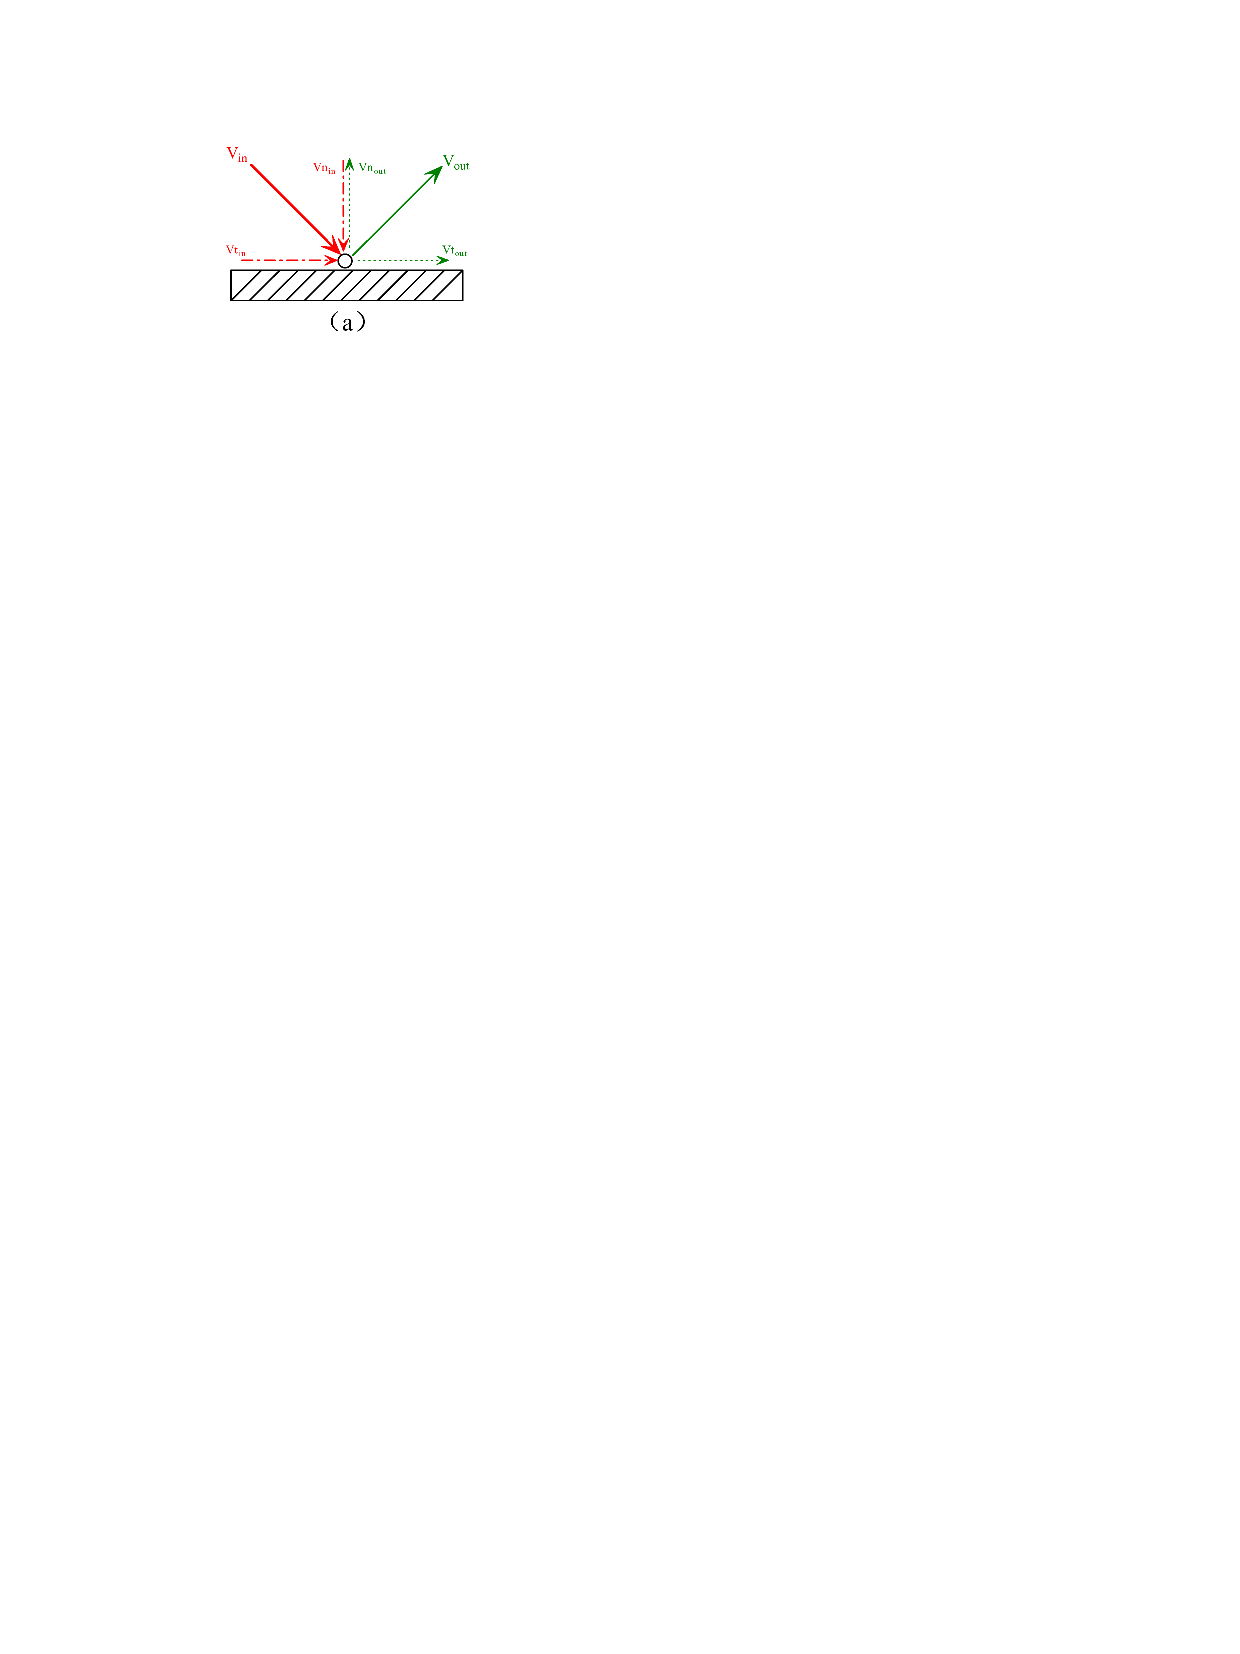
\includegraphics[width=1\textwidth]{./figures/fig02_1.pdf}
\end{center}
\end{column}
\begin{column}[c]{0.25\textwidth}
\begin{center}
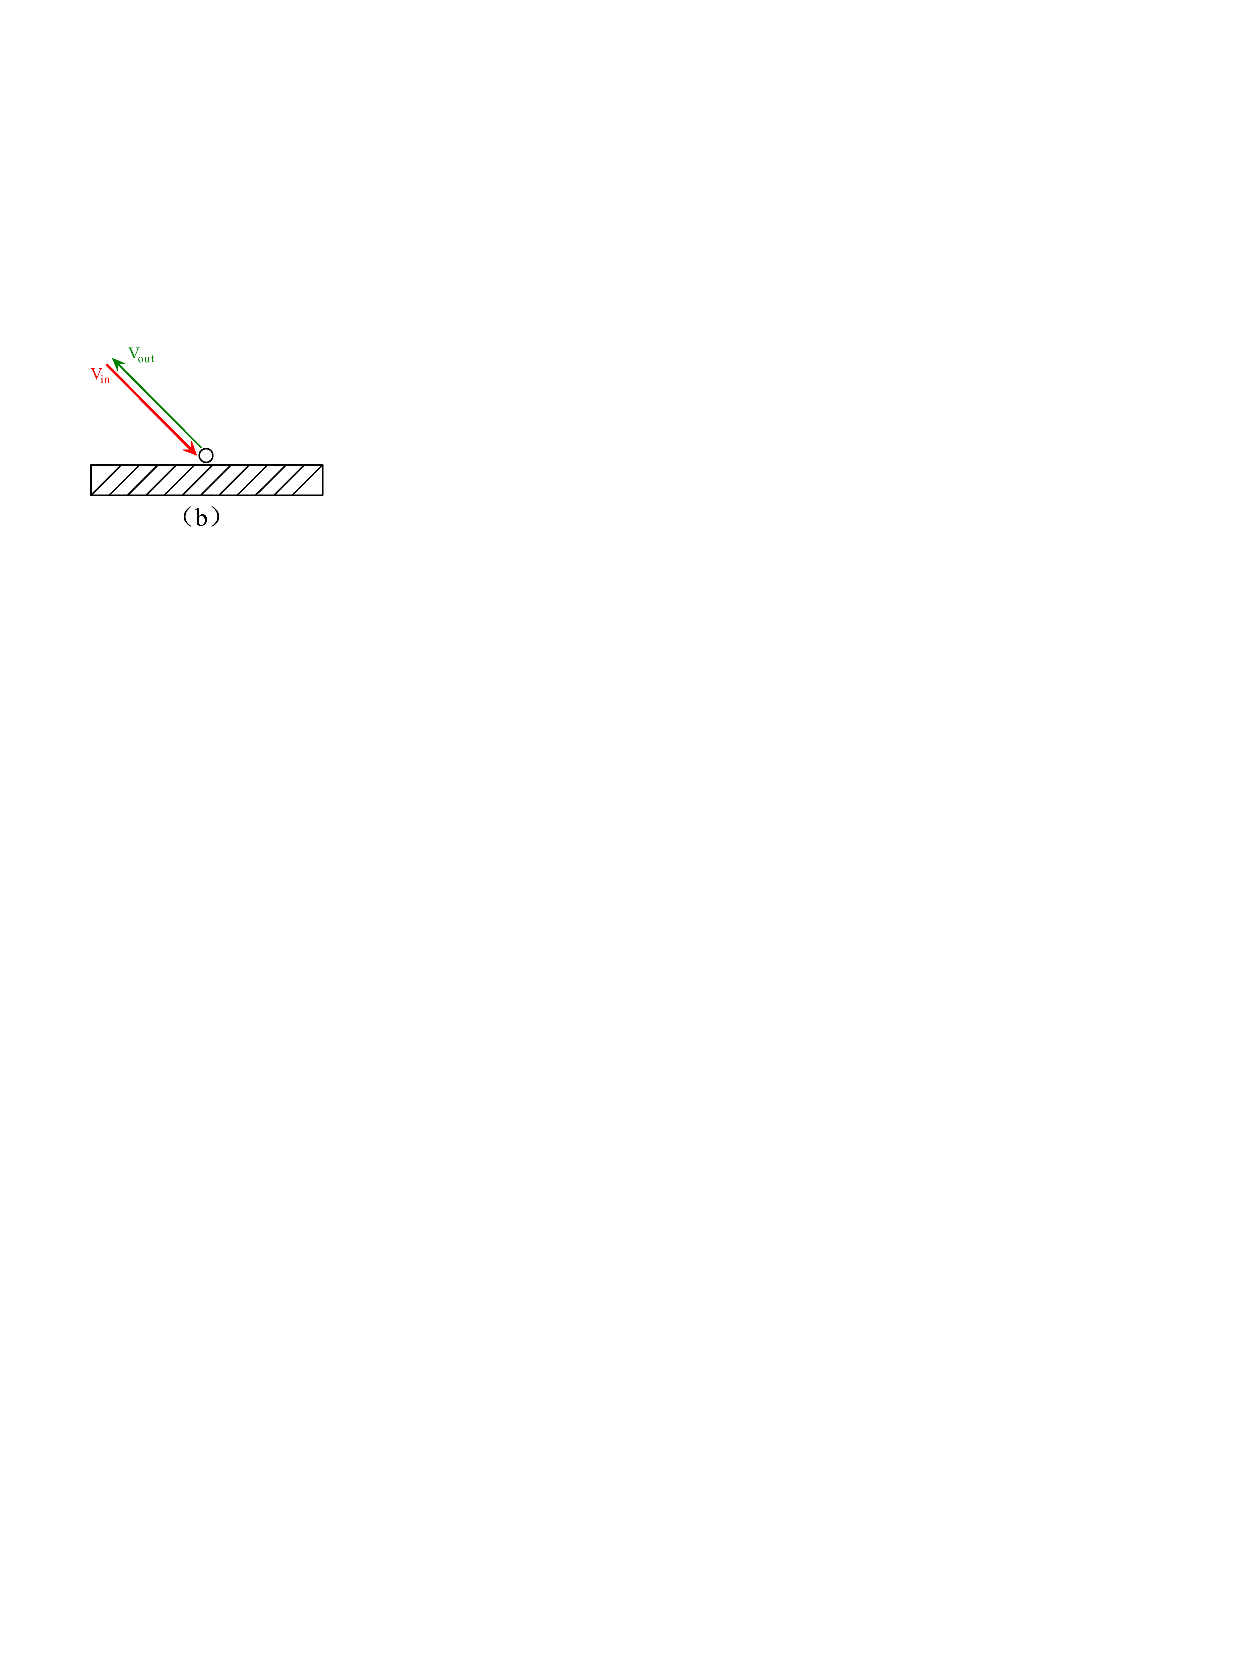
\includegraphics[width=1\textwidth]{./figures/fig02_2.pdf}
\end{center}
\end{column}
\begin{column}[c]{0.25\textwidth}
\begin{center}
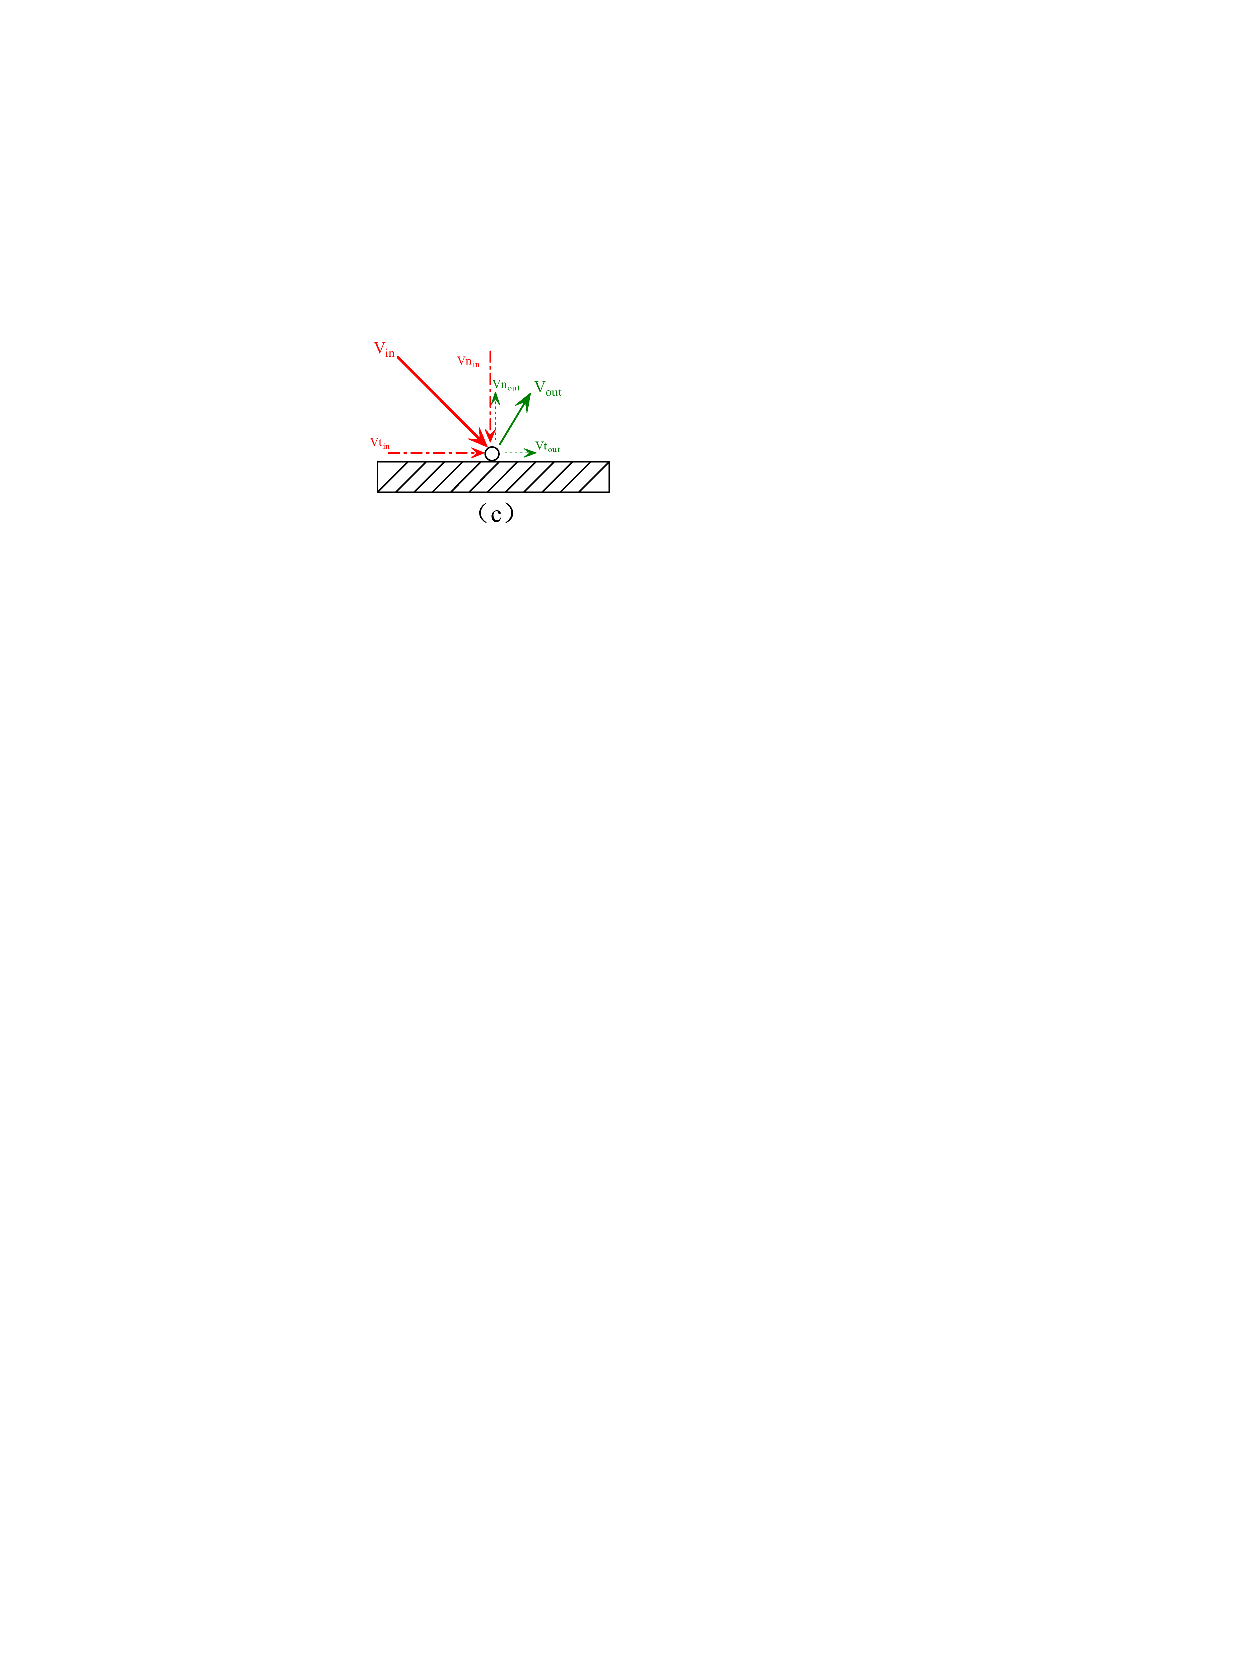
\includegraphics[width=1\textwidth]{./figures/fig02_3.pdf}
\end{center}
\end{column}
\end{columns}
}

\subsection{粒子层与反弹运动方法结合}

\frame{\frametitle{粒子层与反弹运动方法结合}

粒子层与反弹运动方法结合

\begin{center}
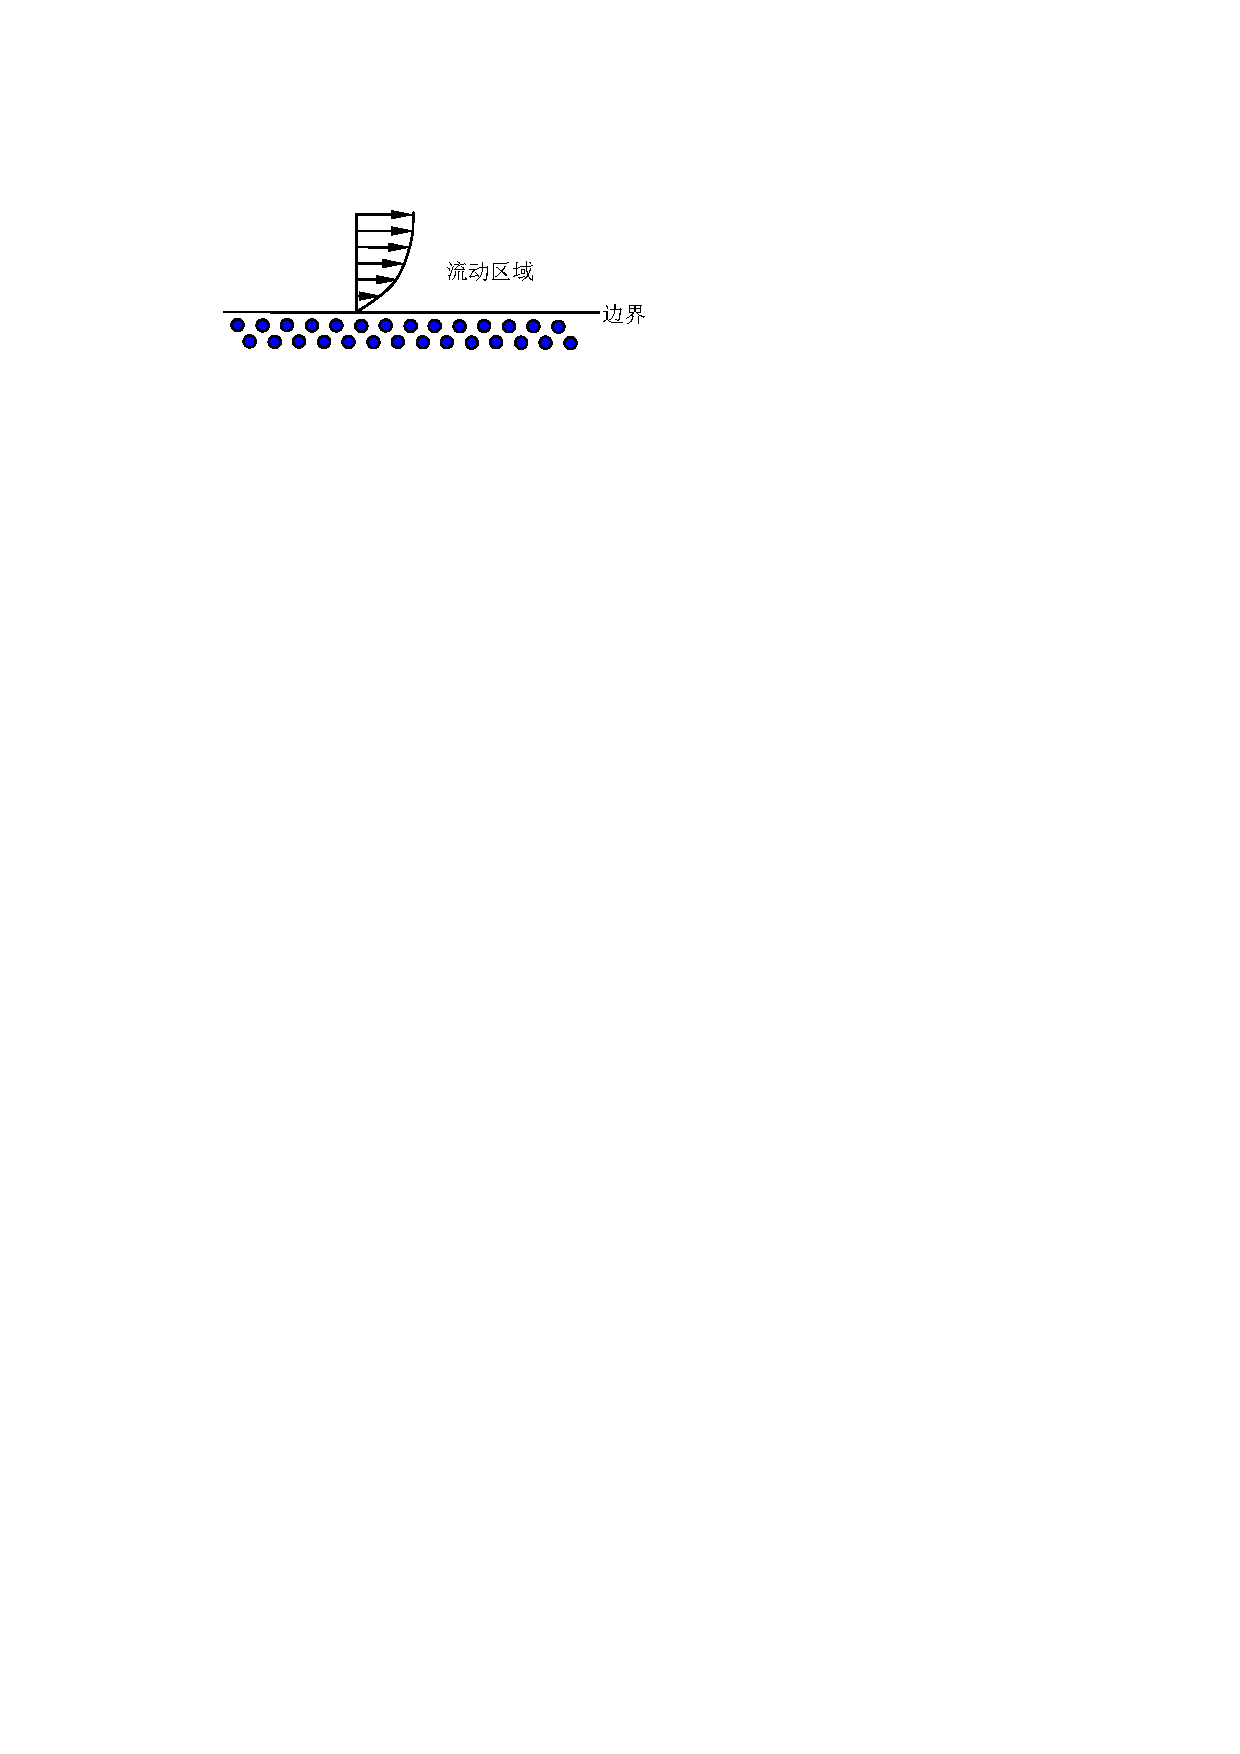
\includegraphics[width=0.7\textwidth]{./figures/fig03.pdf}
\end{center}

}
